\documentclass[conference]{IEEEtran}

\usepackage{cite}
\usepackage{newtxtext,newtxmath}
\usepackage{amsmath}
\usepackage{array}
\usepackage{booktabs}
\usepackage{graphicx}
\usepackage{textcomp}
\usepackage{xcolor}
\usepackage{url}

\newcolumntype{L}[1]{>{\raggedright\arraybackslash}p{#1}}
\newcolumntype{R}[1]{>{\raggedleft\arraybackslash}p{#1}}
\newcommand{\rolebox}[2]{%
  \fcolorbox{black!55}{#1}{\parbox{0.84\columnwidth}{\centering #2}}}

\begin{document}

\title{Evidence-Bound Curation:\\
Auditable Membership Decisions for Language-Model Pretraining Data}

\author{\IEEEauthorblockN{Keonsoo Lee}
\IEEEauthorblockA{\textit{Department of Computer Science} \\
\textit{University of Nevada, Las Vegas}\\
Las Vegas, USA \\
leek133@unlv.nevada.edu}
\and
\IEEEauthorblockN{Shaikh Arifuzzaman}
\IEEEauthorblockA{\textit{Department of Computer Science} \\
\textit{University of Nevada, Las Vegas}\\
Las Vegas, USA \\
shaikh.arifuzzaman@unlv.edu}}

\maketitle

\begin{abstract}
Large-scale data-curation pipelines combine heuristic filters, similarity
retrieval, and learned quality models, but often leave these signals to
directly determine corpus membership. We introduce evidence-bound curation, an
auditable framework for language-model training data that separates evidence
production from the authority to remove data. Validity handles closed input
failures; Redundancy requires an explicit relation and a surviving
representative; Quality positively selects data under declared evidence; and
Coverage may veto removals that extinguish required support but cannot initiate
deletion. Every membership transition is content-addressed and reason-coded,
while downstream evaluation remains outside the curation runtime.

We instantiate the framework on a 6.98M-token Python corpus and construct
Normal and Hard profiles under fixed policies. Hard retains 72.05\% of the Raw
token stream. Across three training seeds and six code benchmarks, Hard reaches
a 20.80 primary reasoning macro compared with 20.86 for Raw, although
benchmark-level changes are mixed. These results demonstrate auditable corpus
compression with near-retained reasoning performance in the evaluated Code
setting. The contribution is a domain-neutral membership-authority framework;
broader downstream effectiveness requires independent validation in additional
domains.
\end{abstract}

\begin{IEEEkeywords}
pretraining data, dataset curation, data quality, auditability, code language
models
\end{IEEEkeywords}

\section{Introduction}
Pretraining-data curation determines not only how much data a model sees, but
which evidence remains available to learning. Large-corpus pipelines routinely
remove malformed content, apply heuristic or learned quality filters, and
deduplicate at exact, fuzzy, or semantic levels
\cite{raffel2020c4,penedo2024fineweb,soldaini2024dolma,li2024datacomp}.
Production tools such as NeMo Curator and Data-Juicer make these operations
configurable and scalable \cite{nvidia2026nemo,chen2023datajuicer}. NeMo's
custom-filter interface usefully separates document scoring from the keep
decision \cite{nvidia2026filtering}, but the recipe author still determines how
heterogeneous decisions compose. That engineering progress exposes a narrower
unresolved question: \emph{when is a signal sufficient to change corpus
membership?}

At large-corpus scale this is a data-systems problem, not merely a scoring
problem: individually plausible operator decisions can compound into millions
of irreversible membership changes whose provenance is difficult to recover
after materialization.

The question matters because the signals are not interchangeable. An absent
payload is an input-contract failure. A MinHash collision is retrieval
evidence, not proof that two programs are equivalent. A classifier abstention
is not a negative quality judgment. Even when individual exclusions are
locally defensible, their union can eliminate the only remaining member of a
support group. A scalar score or ordered list of filters can conceal these
differences behind one keep/drop bit.

Consider two units returned by a MinHash lookup. A similarity-first pipeline
may treat retrieval as permission to discard one unit. Evidence-bound curation
instead treats the pair as a candidate relation: removal is authorized only if
the active policy verifies an allowed relation, records a surviving
representative, and passes the post-composition Coverage recheck. The lookup is
therefore useful without silently acquiring deletion authority. This pattern
extends to learned Quality evidence and semantic support graphs.

We address the problem by separating \emph{evidence} from \emph{decision
authority}. Evidence producers may describe a unit, retrieve comparisons, or
estimate bounded properties, but only a versioned policy may perform a typed
membership transition. Validity, Redundancy, Quality, and Coverage receive
different authority and do not compensate for one another. Coverage is not a
diversity reward or target-mixture optimizer: it is a final veto against
unexplained support extinction. Downstream evaluation is outside the runtime
and begins only after corpus identities are frozen.

Code is a useful stress domain for this separation. Whitespace-only variants
may be equivalent, while a one-token operator, identifier, API signature, or
negation change may alter behavior. Short fragments may be useful despite
lacking execution context. Repository structure also produces long files,
templates, generated artifacts, and source-correlated chunk distributions.
These characteristics make aggressive similarity or scalar-quality shortcuts
easy to state and difficult to defend.

We evaluate the framework along two complementary dimensions. Operational
validation tests whether typed authority prevents unsupported exclusions and
preserves auditable corpus identities after policy composition. Downstream
evaluation measures the compression--capability trade-off when the resulting
profiles are used under their natural token budgets.

This paper makes three contributions:
\begin{itemize}
  \item a typed membership-authority model with machine-checkable invariants
  for trace completeness, surviving representatives, zero-survivor support,
  forbidden inputs, and identity-bound replay;
  \item a concrete A--B--C pipeline combining candidate-only MinHash retrieval,
  survivor-linked redundancy witnesses, an abstention-aware vector Quality
  gate, and veto-only Coverage rematerialization; and
  \item a content-addressed implementation and frozen natural-budget evaluation
  protocol that exposes authority counterfactuals while preventing target size
  or downstream utility from entering curation.
\end{itemize}

The contribution is an executable decision contract that can sit above modern
curation systems providing distributed filtering and deduplication. Its roles
and transition types do not encode Code: evidence producers and versioned
policy artifacts carry domain-specific assumptions. The framework is therefore
language-model general at the authority layer, while the downstream evidence
in this paper qualifies its Code instantiation only. Throughput improvements,
new retrieval algorithms, and production readiness remain outside this claim.

\section{Background and Design Gap}
\subsection{Corpus Construction and Quality Selection}
C4, RefinedWeb, FineWeb, and Dolma document how extraction, language filtering,
content rules, and deduplication shape large language-model corpora
\cite{raffel2020c4,penedo2023refinedweb,penedo2024fineweb,soldaini2024dolma}.
DataComp-LM makes curation recipes comparable under controlled training
protocols \cite{li2024datacomp}. Learned approaches then treat quality as a
selection objective. QuRating learns four scalar ratings from pairwise model
judgments and uses them for sampling and curriculum construction, while D4
combines deduplication with embedding-based diversification
\cite{wettig2024qurating,tirumala2023d4}. Empirical studies further show that a
one-dimensional quality classifier is not sufficient to predict filtering
effects across domains and need not measure an intrinsic notion of document
quality \cite{longpre2024pretrainer,naitsaada2025illusion}.

Our framework complements learned rankers by governing how their evidence may
affect membership. It targets settings in which every change needs a closed
explanation and distinct false-removal risks remain noncompensatory: a Quality
score cannot repair an invalid input or justify eliminating the only surviving
member of a support family.

\subsection{Curation Systems}
Data-Juicer provides composable operators, recipe exploration, tracing, and
evaluation feedback \cite{chen2023datajuicer}. NeMo Curator supplies Ray-based
pipelines, heuristic and model filters, and exact, fuzzy, and semantic
deduplication across multiple modalities \cite{nvidia2026nemo}. Oasis combines
interactive rule filters, a neural filter, adaptive deduplication, and holistic
corpus assessment \cite{zhou2023oasis}. These systems establish operator-level
extensibility and scalable execution. Our focus is orthogonal: a cross-policy
membership-authority contract that can sit above such mechanisms and can be
implemented with their custom stages.

The contract is evaluated through its decision boundaries rather than a
throughput comparison: retrieval supplies candidates, an external teacher
supplies bounded Quality evidence, Coverage supplies only a veto, and external
evaluation receives a materialized corpus without a feedback path. Table~\ref{tab:authority-counterfactuals}
turns these boundaries into executable counterfactuals.

\begin{table*}[t]
\caption{Executable authority counterfactuals. Candidate-edge counts are not
unique would-be deletions; they quantify decisions that the contract refuses
to infer from retrieval alone.}
\label{tab:authority-counterfactuals}
\centering
\footnotesize
\renewcommand{\arraystretch}{1.08}
\setlength{\tabcolsep}{3.5pt}
\begin{tabular}{@{}L{0.16\textwidth}L{0.25\textwidth}L{0.28\textwidth}L{0.23\textwidth}@{}}
\toprule
Shortcut & Unconstrained membership outcome & Evidence-bound restriction & Frozen audit result \\
\midrule
Retrieval as deletion & Similarity candidates become removable duplicate-family members & Typed relation witness and final surviving representative & Normal $2{,}515\rightarrow2$; Hard $2{,}873\rightarrow3$ \\
Local selection only & Threshold-not-met units disappear even when a support group reaches zero survivors & Coverage has veto-only restore authority followed by full recheck & 99 Normal and 429 Hard chunks restored \\
Stale evidence reuse & A changed text, provider, policy, or threshold inherits an earlier decision & Every consumed artifact is identity- and hash-bound & All exercised identity mutations rejected \\
Evaluation feedback & A favorable or adverse score retunes membership after observing outcomes & Evaluator fields are absent from selector inputs; corpus hashes freeze first & 60 cells observed with zero feedback path \\
\bottomrule
\end{tabular}
\end{table*}

\subsection{Deduplication for Code}
Deduplication can reduce memorization and evaluation leakage
\cite{lee2022deduplicating}. The Stack applies responsible source-code dataset
construction and near-deduplication \cite{kocetkov2023stack}. MinHash and LSH
efficiently retrieve high-overlap candidates \cite{broder1997resemblance}, but
overlap is especially ambiguous for code. Two files can share imports and
structure while implementing different behavior, and pairwise near relations
need not be transitive. We therefore use similarity only to decide which pairs
receive a deterministic relation test. It never supplies membership authority
by itself.

\subsection{Two Failure Patterns}
Two composition failures motivate the contract. Functions differing only in
\texttt{return x >= 0} versus \texttt{return x > 0} may collide in many LSH
bands although neither represents the other; retrieval must therefore open a
comparison rather than authorize deletion. Conversely, every member of a
partial-fragment group may lack enough local Q1 evidence without being known
incorrect. Materializing those local non-selections can silently erase the
group, so Coverage alone may require a representative. The first case
over-authorizes similarity and the second over-interprets missing positive
evidence. Table~\ref{tab:authority-counterfactuals} makes both failure modes
executable rather than leaving them as pipeline-order advice.

\section{Evidence-Bound Membership Model}
\subsection{Evidence, Policy, and Authority}
Let $D$ be an audited input corpus and $U(D)$ the deterministic training units
created from it. A profile $m$ materializes $C_m\subseteq U(D)$ together with a
trace $T_m$. For a unit $x$, an evidence producer emits an observation
$e=(x,h_x,p,v,r)$ containing the unit identity, text hash, producer, version,
and result. An observation is descriptive until an authorized policy maps it
to a typed state transition.

The model recognizes four non-compensatory roles:
\begin{enumerate}
  \item \textbf{Validity} may quarantine a closed input-contract failure.
  \item \textbf{Redundancy} may propose removal of a nonrepresentative only
  with an authorized relation witness and surviving representative.
  \item \textbf{Quality} may positively select a unit under independent
  Q1--Q4 evidence; insufficient positive evidence is recorded as
  \emph{not selected}, not as proof that the unit is useless.
  \item \textbf{Coverage} may veto the combined proposals and require explicit
  rematerialization; it cannot create a new exclusion.
\end{enumerate}

Figure~\ref{fig:authority} shows the separation. The boundary is asymmetric:
uncertain Redundancy evidence retains, whereas uncertain Quality evidence does
not count as a positive pass. Both behaviors are explicit policy choices, not
implicit consequences of one global score.

\begin{figure}[t]
\centering
\footnotesize
\rolebox{blue!6}{\textbf{Evidence producers}\\
input checks; digests and MinHash retrieval; local Q1--Q4 ranker;
semantic support graph}
\\[-1pt]$\downarrow$\\[-1pt]
\rolebox{green!7}{\textbf{Membership authority}\\
Stage A quarantine; Stage B witnessed redundancy and positive selection;
Stage C veto-only restore}
\\[-1pt]$\downarrow$\\[-1pt]
\rolebox{gray!10}{\textbf{Frozen corpus identity}\\
stable IDs, policy and evidence hashes, reason codes,
representative/restore links}
\\[-1pt]$\downarrow$\\[-1pt]
\rolebox{orange!9}{\textbf{External validation only}\\
continued pretraining and benchmarks; no path back to membership}
\caption{Evidence can reach corpus membership only through the authority shown
for its role. The external experiment observes frozen outputs and has no
selector input path.}
\label{fig:authority}
\end{figure}

\subsection{Required Invariants}
For each membership-changing proposal $p(x)$, the trace must contain a valid
policy artifact $\pi$, evidence $e$, and text identity $h_x$:
\begin{equation}
p(x)\Rightarrow
\mathrm{valid}(\pi,e,h_x)\land\mathrm{authorized}(\pi,e,x,m).
\label{eq:authority}
\end{equation}
For Redundancy, $p(x)$ additionally names a representative $s(x)$ and witness
$w(x,s)$, with $s(x)$ surviving final materialization. Missing evidence cannot
be replaced by a run-local heuristic. A changed tokenizer, normalization,
provider, model artifact, threshold, or schema invalidates inherited evidence.

Let $V$ be Stage B-eligible units and $P_m$ the reason-coded Stage B
non-selection set. The provisional corpus is
$\widetilde C_m=V\setminus P_m$. For every active support group $g$, Coverage
requires either a survivor or an authorized zero-survivor explanation $a_g$:
\begin{equation}
I_g(\widetilde C_m)=
\mathbf{1}[g\cap\widetilde C_m\neq\emptyset\ \lor\ a_g=1].
\label{eq:coverage}
\end{equation}
If any $I_g=0$, Stage C emits required-retain IDs $R_m$, writes
$C_m=\widetilde C_m\cup R_m$, and reruns the complete invariant set. No
weighted average allows one intact group to compensate for another group's
extinction.

\subsection{Executable Contract Invariants}
An accepted materialization exposes five checks already enforced by the
runtime contract. Every membership change must emit a complete
\emph{reason-coded trace} naming its policy, observable evidence, action, and
text identity. Every Redundancy exclusion must pass
\emph{representative survival}. Coverage runs the declared
\emph{zero-survivor check} and emits explicit required-retain IDs when support
would otherwise disappear. The \emph{forbidden-input check} rejects selector
access to downstream outcomes. Finally, \emph{identity-bound replay} requires
identical bound artifacts for resume and rejects inherited evidence after a
text, provider, policy, or threshold identity changes.

\textbf{Proposition 1 (contract-checked materialization).} Assume deterministic
unitization and policy execution, collision-resistant content identities, and
complete trace emission. Any transaction accepted by the final recheck
satisfies the five invariants above; in particular, retrieval-only deletion,
representative-free Redundancy removal, unexplained support extinction,
evaluation-driven reselection, and stale-evidence replay cannot be accepted.

\emph{Proof sketch.} Induct over the ordered transition log. Stage A can emit
only a closed Validity quarantine. Every Stage B removal is admitted by the
role-specific policy and records the evidence and current text hash;
Redundancy additionally records a survivor checked against final membership.
Stage C forms only $\widetilde C_m\cup R_m$ and reruns Eq.~\eqref{eq:coverage},
so it cannot originate an exclusion. The external evaluator is downstream of
the frozen corpus hash and has no selector field. Finally, any changed bound
identity aborts resume before a transition is consumed. These cases exhaust
the membership-changing transitions in the contract. The proposition is a
property of accepted executions under the stated assumptions, not a claim
that an implementation is free of arbitrary software defects.

The distinction between \emph{rejected} and \emph{not selected} remains part
of the trace. Validity and witnessed Redundancy carry closed negative evidence;
a Quality threshold-not-met state says only that the profile lacks sufficient
positive Q1--Q4 evidence. No role may borrow another role's signal to
compensate for a failed precondition.

\subsection{Forbidden Feedback}
The curation runtime is intentionally unable to read benchmark outcomes,
pretraining loss, NLL, a utility estimate, source reputation, source tier,
target domain shares, a retention fraction, or a maximum token budget. These
values can describe or evaluate a frozen output, but cannot alter that output.
This is stronger than promising not to tune on a benchmark: the forbidden
inputs are absent from the active policy configuration and reported as unread
in materialization artifacts.

\section{Curation Pipeline}
\subsection{Stage A: Closed Validity}
The input adapter preserves declared metadata without inferring missing rights
or provenance. Stage A normalizes only payload-preserving representation and
quarantines observable contract failures: absent text, a declared text-contract
violation, unrecoverable corruption, or acquisition failure. Short code,
partial files, unfamiliar formats, markup, multilingual text, and parser
failure remain valid by default. Rights, PII, poisoning, and source-admission
review are separate audit concerns; they are not silently converted into a
text-quality score.

Released records are chunked deterministically into units of at most 6,000 characters.
Every chunk retains its parent record ID and normalized text hash. Stage B
first removes normalized exact duplicates, before candidate retrieval or
model-assisted Quality is considered.

\subsection{Stage B: Witnessed Redundancy}
Candidate retrieval combines exact text and formatting digests, exact
containment-window digests, and MinHash LSH. The active retrieval settings are
5-token shingles, a 32-value signature, eight bands, and a 24-token retrieval
minimum. Normal admits bounded-near comparisons from 96 tokens with at most
two changed tokens and 1\%; Hard uses 64 tokens, four changes, and 2\%.
Units of at most 32 tokens are exact-only.

Retrieval only schedules comparisons. An exclusion proposal requires an
authorized typed witness: exact text, formatting equivalence, bounded near
substitution, token-preserving prose reflow, exact token containment, or, in
Hard, a declared equivalence verifier. Numeric, operator, negation, answer
label, API-signature, code-identifier/keyword, and named-entity changes trigger
substantive-difference protection. Near edges remain pairwise and are not
transitively closed. A payload superset is preferred as representative, with a
stable ID tie break.

This split between retrieval and decision is essential to the paper's claim.
The frozen run evaluated thousands of candidate pairs, yet every authorized
redundancy exclusion was justified by exact token containment rather than
MinHash similarity alone (Section~\ref{sec:materialization}).

\subsection{Stage B: Structural Non-Payload Rules}
Four closed text rules detect an explicit generated-and-do-not-edit artifact,
a license-comment-only chunk, an empty HTML shell, or a chunk containing only
a fixed vocabulary of web controls. Each requires positive in-text evidence.
A generated source label alone, ordinary documentation, code with a license
header, prose about cookies, and HTML with visible or executable content are
protected negative cases. Candidate span transformations are disabled in the
frozen Normal and Hard runs; consequently, all selected chunks are exact
substrings of their parent records.

\subsection{Stage B: Distilled Vector Quality}
Quality is an evidence vector, not an intrinsic scalar:
\begin{equation}
Q(x)=(Q_1,Q_2,Q_3,Q_4),\qquad Q_i\in\{P,F,A\},
\label{eq:quality}
\end{equation}
where $P$, $F$, and $A$ denote pass, fail, and abstain. The heads ask whether
the unit has (Q1) locally observable correctness evidence, (Q2) semantic
coherence, (Q3) substantive payload, and (Q4) at least one learnable relation.
A head fails only on its closed reason codes. Missing external knowledge,
undeclared execution assumptions, missing context, specialized notation,
low confidence, and out-of-distribution input abstain.

GPT-5.6 Luna supplies offline Q1--Q4 labels through a versioned Batch
configuration. It does not process the full corpus and its output alone may
neither select nor exclude a chunk. The fitting pool combines 1,024 corpus
chunks with 576 policy-targeted synthetic enrichment fixtures (144 per head),
giving each head 1,168 labeled observations before its fit/calibration split.
A UID- and text-hash-disjoint protected set contains 800 corpus chunks. The
local four-head ranker uses Qwen3-Embedding-0.6B representations, the same
encoder and heads for both profiles, minimum decision confidence 0.8, and OOD
cosine-similarity threshold 0.3822.

Let $P(x)$ be the confident in-distribution heads predicting pass and $F_m(x)$
the qualified fails at operating point $m$. The selection rules are
\begin{align}
\mathrm{Select}_{N}(x)&=\mathbf{1}[|P(x)|\geq1\land |F_N(x)|=0],\\
\mathrm{Select}_{H}(x)&=\mathbf{1}[|P(x)|\geq2\land |F_H(x)|=0].
\label{eq:selection}
\end{align}
Abstention supplies no positive selection evidence. Therefore a chunk that
does not meet the pass count is recorded as threshold-not-met, not as a
qualified failure or a claim of universal uselessness. Stage C may later
restore it only through a typed Coverage veto.

\subsection{Stage C: Veto-Only Coverage}
Coverage evaluates the combined Stage B result over nonexclusive views:
redundancy families, deterministic content routes, language/script and format
labels, residual links, and semantic support strata. The frozen semantic graph
uses Qwen3-Embedding-0.6B as its primary provider and BGE-M3 as an independent
audit view \cite{zhang2025qwen3embedding,chen2024bgem3}. Mutual eight-neighbor
relations shared by both views define stable local support; provider-specific
neighborhoods remain uncertainty strata. Embedding similarity never authorizes
an exclusion.

When a provisional output leaves a group unexplained and empty, Coverage
chooses a deterministic representative, records why it is required, restores
it, and performs a second complete check. Hard restoration candidates are
bounded by final Normal membership, enforcing
\begin{equation}
C_{\mathrm{Hard}}\subseteq C_{\mathrm{Normal}}.
\end{equation}
Coverage does not maximize a diversity score, impose a quota, or infer that a
rare group is useful. Its claim is narrower: membership loss must be accounted
for, and an unexplained extinction blocks materialization.

\subsection{Audit Trace}
Each boundary writes stable unit and parent IDs, original and evidence hashes,
policy/provider versions, discrete decisions, reason codes, and any
representative or required-retain link. The top-level report aggregates token
and chunk impact by reason and checks representative survival, subset
invariants, residual identity, and complete Coverage recheck. Composition is
reported only between Stage B eligibility and the Stage C output so the unit
and denominator remain comparable.

Materialization is executed as a transaction:
\begin{enumerate}
  \item validate source, tokenizer, policy, model, and schema identities;
  \item release or quarantine records under Stage A and deterministically
  create chunk identities;
  \item retrieve Redundancy candidates, evaluate typed witnesses, apply closed
  non-payload rules, and run the version-bound local Q1--Q4 ranker;
  \item write the complete provisional membership set and all reason traces;
  \item evaluate every Coverage view, emit required-retain IDs, explicitly
  rematerialize, and rerun the complete invariant set; and
  \item hash the final corpus and only then expose it to the external training
  protocol.
\end{enumerate}
An interrupted run may resume only when every bound identity matches. A stale
or corrupt cache reduces usable evidence or aborts the transaction; it cannot
activate a looser fallback. This recovery rule makes reproducibility a
membership property rather than a best-effort logging feature.

\begin{table}[t]
\caption{Authority and fail-closed behavior in the implemented pipeline.}
\label{tab:authority}
\centering
\footnotesize
\renewcommand{\arraystretch}{1.08}
\setlength{\tabcolsep}{2.5pt}
\begin{tabular}{@{}L{0.17\linewidth}L{0.47\linewidth}L{0.22\linewidth}@{}}
\toprule
Role & Authorized action & Fallback \\
\midrule
Validity & Quarantine a closed contract failure & Release on ambiguity \\
Redund. & Propose witnessed removal; link survivor & Retain pair \\
Quality & Select on pass count and no qualified fail & No positive pass \\
Coverage & Veto and explicitly restore support & Never excludes \\
External eval. & Measure a frozen corpus/model arm & No feedback path \\
\bottomrule
\end{tabular}
\end{table}

\section{Implementation}
\subsection{Content-Addressed Execution}
The implementation separates policy specification, evidence artifacts, and
materialization. JSON contracts bind the source manifest, tokenizer, chunking,
model and provider identities, operating points, and output locations. A
runtime bridge rejects a resume if a bound identity or content hash changes.
The final Normal and Hard configurations use the same active policy families;
only versioned Redundancy bounds and the required Quality pass count differ.

Table~\ref{tab:implementation} lists settings that materially affect
membership. Luna is absent from the full-corpus execution row because it is an
offline calibration oracle. Likewise, Qwen3-4B-Base appears only in external
training, never as a selector feature.

\begin{table}[t]
\caption{Versioned implementation settings that affect membership.}
\label{tab:implementation}
\centering
\footnotesize
\renewcommand{\arraystretch}{1.08}
\setlength{\tabcolsep}{3pt}
\begin{tabular}{@{}L{0.22\linewidth}L{0.70\linewidth}@{}}
\toprule
Component & Setting \\
\midrule
Identity & Stable UID, parent UID, normalized text/evidence SHA-256 \\
Chunking & Format preserving; maximum 6,000 characters \\
Retrieval & Exact/format/containment digests; 5-token shingles; 32-value MinHash; eight LSH bands \\
Redundancy & Exact-only through 32 tokens; Normal $\geq96$ tokens, $\leq2$ changes/1\%; Hard $\geq64$, $\leq4$/2\% \\
Non-payload & Four closed in-text rules; no active span transformation \\
Quality & Qwen3-Embedding-0.6B; confidence $\geq0.8$; OOD cosine $\geq0.3822$; Normal $\geq1$ pass, Hard $\geq2$ \\
Qualified fail & Q1/Q3 fail off; Q2 Normal/Hard $0.4236/0.2032$; Q4 $0.8150/0.3602$ \\
Coverage & Qwen3 embedding primary, BGE-M3 audit view; mutual eight-neighbor support graph; veto only \\
Selector inputs & Text and authorized evidence only; no utility, loss, benchmark, source, quota, or token budget \\
\bottomrule
\end{tabular}
\end{table}

\subsection{Policy Qualification Boundary}
The distilled ranker is a candidate policy component. Its
1,024-dimensional encoder representation, four heads, OOD boundary, and
protected-set threshold checks are inspectable. Q1 and Q3 have no promoted
fail threshold; Q2 and Q4 alone use protected-set-verified fail thresholds.
The evaluated corpus records no qualified Quality failure, so its profile
difference comes from one-pass versus two-pass positive selection. We treat
this as a fixed Code-corpus operating point, not as a universal quality
classifier.

Accordingly, the paper reports two evidence levels: executable conformance of
the membership transaction and a bounded Code-domain materialization and
training study. Production release and cross-domain promotion remain outside
the present evidence; they are not prerequisites for testing the proposed
decision contract.

\subsection{Conformance Evidence}
Fixtures exercise positive, false-positive, adversarial, and metamorphic paths.
Corpus reports then verify typed Quality decisions, final representatives,
veto-only Stage C, complete recheck, and the Hard-subset-of-Normal invariant;
source, leakage, and packed-input reports bind hashes and exact token, block,
and step counts. These checks establish executable conformance, not corpus-wide
semantic accuracy or downstream benefit.

The frozen semantic artifact records 3,843 stable strata, 2,830 uncertainty
strata, and 23,636 pairwise entries under two provider identities. Normal and
Hard bind the same graph hash and every required-retain UID. These are the
support views Stage C consumed, not an estimate of their semantic precision.

\begin{table*}[t]
\caption{Frozen natural-budget materialization. Unit types differ between Raw
(records) and curated arms (chunks); stream and packed tokens use the same
Qwen3-4B tokenizer.}
\label{tab:materialization}
\centering
\footnotesize
\renewcommand{\arraystretch}{1.08}
\setlength{\tabcolsep}{3.5pt}
\begin{tabular}{@{}L{0.18\textwidth}R{0.11\textwidth}R{0.115\textwidth}R{0.115\textwidth}R{0.115\textwidth}R{0.08\textwidth}R{0.07\textwidth}@{}}
\toprule
Arm & Units & Stream tokens & Packed tokens & Stream retention & Blocks & Steps \\
\midrule
Raw audited & 4,890 records & 6,984,438 & 6,979,584 & 100.00\% & 3,408 & 426 \\
Normal & 7,147 chunks & 6,125,213 & 6,111,232 & 87.70\% & 2,984 & 373 \\
Hard & 5,859 chunks & 5,032,400 & 5,029,888 & 72.05\% & 2,456 & 307 \\
\bottomrule
\end{tabular}
\end{table*}

\section{Evaluation}
\subsection{Corpus and Exclusion Boundary}
The frozen Raw arm is a mixed Python-code corpus, not a purely raw Stack
sample. It contains 4,228 records and 4,723,925 Qwen3-4B stream tokens
(67.64\%) from \texttt{bigcode/the-stack-dedup}, plus 662 records and
2,260,513 tokens (32.36\%) from version-pinned snapshots of eight established
open-source repositories. The final total is 4,890 records and 6,984,438
stream tokens including one EOS per record.

Before curation, an exclusion audit compared 4,902 candidates with frozen
snapshots of HumanEval+, MBPP+, LiveCodeBench Code Generation Lite,
BigCodeBench Complete, CRUXEval-I/O, and DS-1000. It excluded 12 records using
exact normalized segments or shared 16-token shingles. This establishes only
the declared exact/shingle boundary; it does not prove absence of semantic,
translated, shorter, or base-model contamination.

Calibration and protected Quality samples are UID- and text-hash-disjoint from
each other but drawn from the same 8,024-chunk corpus. Corpus-wide
materialization then uses the frozen local ranker. The external teacher is not
queried, and all configuration reports state that benchmark, utility, and
token-budget inputs were unread.

\subsection{Natural-Budget Continued Pretraining}
We continue Qwen3-4B-Base \cite{yang2025qwen3} on audited Raw, Normal, and Hard.
Each arm uses its complete natural token stream; there is no equal-token
resampling, target retention fraction, or maximum-token cap. Seeds are 101,
202, and 303. Training uses sequence length 2,048, micro-batch size 1,
gradient accumulation 8, learning rate $5\times10^{-5}$, weight decay 0.1,
gradient clipping 1.0, and QLoRA rank 32, alpha 64, and dropout 0.05 over all
linear target modules. Adapter training uses 4-bit NF4 weights, double
quantization, and bfloat16 compute. Only the final incomplete sequence and
accumulation group are dropped. The model and tokenizer are bound to revision
\texttt{906bfd4b4dc7f14ee4320094d8b41684abff8539}. Optimization uses AdamW
with betas $(0.9,0.999)$, epsilon $10^{-8}$, a constant learning rate, and no
scheduler or warmup.

All reported scores use deterministic pass@1 generation. Prompts are tokenized
without added special tokens; decoding is greedy and stops at EOS or the
suite-specific maximum: 512 new tokens for EvalPlus, 1,024 for BigCodeBench
and DS-1000, and 256 for CRUXEval. EvalPlus, BigCodeBench, and DS-1000 use the
same code-fence/terminal-marker trimming rule; CRUXEval uses its canonical
direct prompts and upstream task-specific postprocessing. Scoring binds
EvalPlus 0.3.1, BigCodeBench v0.1.4 and its public Complete evaluator, CRUXEval
commit \texttt{190faf1}, and DS-1000 commit \texttt{b39aab7}. The frozen
protocol, packed-input report, generated task IDs, scorer outputs, and all 60
cell hashes are retained in the accompanying manifest package.

The primary reasoning suite is BigCodeBench Complete, CRUXEval-I, CRUXEval-O,
and DS-1000. HumanEval+ and MBPP+ are mandatory secondary short-function
diagnostics \cite{liu2023evalplus,zhuo2025bigcodebench,gu2024cruxeval,
lai2023ds1000}. The hierarchy was timestamp-frozen after all HumanEval+ and
partial MBPP+ results and Base-only CRUXEval observations, but before any
non-Base result on the primary suite. This is a post-EvalPlus,
pre-primary-results analysis amendment, not a preregistered endpoint. All arms,
seeds, and six benchmarks remain reportable. The
primary summary is the unweighted macro of the four benchmark percentages
after seed aggregation. No arm or seed may be omitted because of its outcome,
and the two secondary diagnostics remain visible even when they disagree with
the primary summary.

% FINAL_RESULTS_BLOCK_BEGIN
\begin{table*}[t]
\caption{Artifact-audited benchmark scores (\%). Trained-arm columns report
seeds 101, 202, and 303 separately. The final row reports the three-seed
primary-macro mean$\pm$sample standard deviation; no best-seed selection is
used.}
\label{tab:downstream}
\centering
\footnotesize
\renewcommand{\arraystretch}{1.10}
\setlength{\tabcolsep}{3pt}
\begin{tabular}{@{}L{0.145\textwidth}R{0.055\textwidth}*{9}{R{0.070\textwidth}}@{}}
\toprule
Benchmark & Base & \multicolumn{3}{c}{Raw} & \multicolumn{3}{c}{Normal} & \multicolumn{3}{c}{Hard} \\
\cmidrule(lr){3-5}\cmidrule(lr){6-8}\cmidrule(lr){9-11}
& & 101 & 202 & 303 & 101 & 202 & 303 & 101 & 202 & 303 \\
\midrule
HumanEval+ & 31.10 & 30.49 & 28.66 & 27.44 & 32.93 & 32.93 & 29.27 & 29.88 & 32.93 & 29.27 \\
MBPP+ & 58.47 & 45.50 & 50.00 & 51.32 & 54.76 & 52.65 & 53.70 & 54.76 & 54.76 & 53.97 \\
BigCodeBench & 39.91 & 40.35 & 41.84 & 40.79 & 40.18 & 38.95 & 39.39 & 39.12 & 40.09 & 40.35 \\
CRUXEval-I & 3.50 & 6.38 & 7.63 & 7.50 & 8.75 & 5.50 & 4.75 & 5.63 & 6.25 & 6.63 \\
CRUXEval-O & 2.13 & 2.88 & 2.00 & 1.38 & 5.63 & 3.25 & 5.00 & 5.38 & 5.25 & 4.13 \\
DS-1000 & 28.00 & 33.10 & 33.60 & 32.90 & 31.60 & 32.20 & 31.90 & 31.10 & 33.00 & 32.70 \\
\midrule
\textbf{Primary macro} & \textbf{18.38} & \textbf{20.68} & \textbf{21.27} & \textbf{20.64} & \textbf{21.54} & \textbf{19.97} & \textbf{20.26} & \textbf{20.31} & \textbf{21.15} & \textbf{20.95} \\
\textbf{Mean $\pm$ SD} & -- & \multicolumn{3}{c}{\textbf{20.86 $\pm$ 0.35}} & \multicolumn{3}{c}{\textbf{20.59 $\pm$ 0.83}} & \multicolumn{3}{c}{\textbf{20.80 $\pm$ 0.44}} \\
\bottomrule
\end{tabular}
\end{table*}
% FINAL_RESULTS_BLOCK_END

\begin{figure*}[t]
\centering
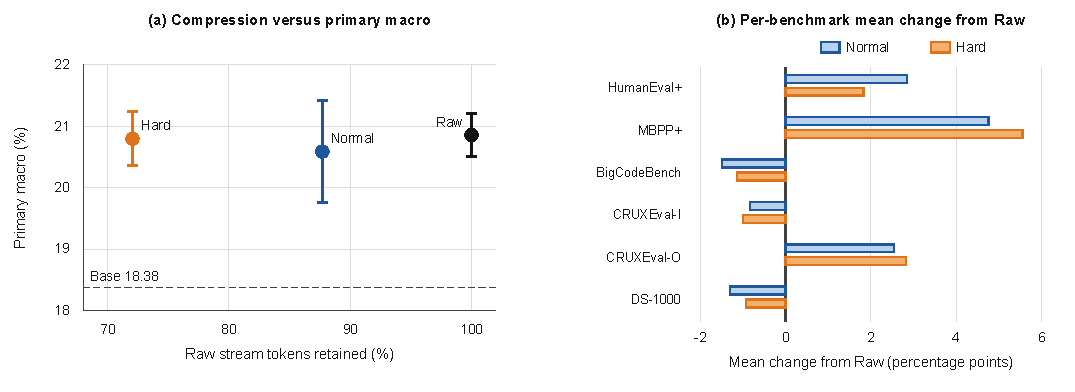
\includegraphics[width=\textwidth]{figures/results_tradeoff.pdf}
\caption{Compression and capability trade-offs. Panel (a) reports three-seed
means with sample-standard-deviation error bars; Base is a no-update reference,
not a zero-token training arm. Panel (b) reports descriptive mean differences.
Neither panel is a significance or non-inferiority test.}
\label{fig:results-tradeoff}
\end{figure*}

\subsection{Operational Validation}
\label{sec:materialization}
Table~\ref{tab:materialization} records the materialized corpora used by every
downstream run. Raw unit count is a record count, while Normal and Hard are
chunk counts; only token columns support direct size comparison. Normal retains
87.70\% of Raw stream tokens and Hard retains 72.05\%. Packed tensors contain
2,984 and 2,456 sequences respectively, compared with 3,408 for Raw.

Table~\ref{tab:mechanism} exposes the decision path. Stage A released 4,889 of
4,890 records, and Stage B produced 8,024 eligible chunks after one exact
duplicate rejection. The closed structural rules removed 39 explicit
generated artifacts and one license-comment-only chunk in each profile.
Normal evaluated 2,515 redundancy candidate pairs and authorized two
containment removals; Hard evaluated 2,873 and authorized three. All had stable
representatives, and no removal was authorized solely by MinHash, a semantic
neighbor, or a transitive near-duplicate component.

The Quality stage is a positive-selection gate. Normal selected 7,048 chunks
before Coverage and recorded 934 as threshold-not-met. Hard selected 5,430 and
recorded 2,551 as threshold-not-met. In both profiles only 25 chunks passed all
four heads, and almost every chunk contained at least one abstention. The run
recorded no qualified fail. Those facts prevent an incorrect interpretation of
the nonselected set as a measured set of bad programs.

Stage C restored 99 Normal and 429 Hard chunks. Both outputs then passed the
complete recheck, no transformation was applied, and Hard remained an exact
UID subset of Normal. The restore counts directly demonstrate that the
Coverage path was active rather than decorative; they do not by themselves
establish that every restored semantic group improves downstream performance.

The counterfactuals expose why the operators alone are not the contribution.
Of 2,515 Normal and 2,873 Hard retrieved Redundancy pairs, only two and three
respectively satisfied an authorized relation witness. Thus, 2,513 and 2,870
candidate edges remained evidence for comparison rather than silently becoming
membership decisions; these are edge counts, not unique would-be deletions.
Without the Stage C veto, 99 Normal and 429 Hard required-retain units would be
absent from provisional membership and the declared support invariant would
fail. Finally, the identity-mutation checks reject inherited evidence rather
than resuming under a changed text, provider, policy, or threshold identity.

\begin{table}[t]
\caption{Mechanism audit for the frozen Normal and Hard outputs.}
\label{tab:mechanism}
\centering
\footnotesize
\renewcommand{\arraystretch}{1.07}
\setlength{\tabcolsep}{3.5pt}
\begin{tabular}{@{}L{0.55\linewidth}R{0.17\linewidth}R{0.17\linewidth}@{}}
\toprule
Measure & Normal & Hard \\
\midrule
Stage B-eligible chunks & 8,024 & 8,024 \\
Structural non-payload exclusions & 40 & 40 \\
Redundancy candidate pairs & 2,515 & 2,873 \\
Witnessed redundancy exclusions & 2 & 3 \\
MinHash-only authorized exclusions & 0 & 0 \\
Quality threshold-not-met & 934 & 2,551 \\
Quality-selected before Coverage & 7,048 & 5,430 \\
Coverage required-retain IDs & 99 & 429 \\
Final chunks & 7,147 & 5,859 \\
Unexplained extinction after recheck & 0 & 0 \\
Active text transformations & 0 & 0 \\
\bottomrule
\end{tabular}
\end{table}

\subsection{Source and Composition Effects}
Source identity was not exposed to the selector, yet retention is
source-correlated. Normal retains 85.64\% of Stack tokens and 92.00\% of
reference-pool tokens; Hard retains 69.40\% and 77.59\%, respectively.
Reference records are also longer (median 6,283 versus 2,039 characters), so
they account for 25.61\% of Stage B chunks despite being 13.54\% of Raw
records. We report record, chunk, and token denominators separately and do not
infer a causal source-quality effect.

Using the comparable chunk view from Stage B eligibility to the Stage C output,
the exclusive primary
route distribution moves only modestly. Code-artifact share is 49.90\% at
eligibility, 49.84\% in Normal, and 49.56\% in Hard; mixed code/prose is
43.42\%, 44.33\%, and 44.46\%; general prose is 5.61\%, 4.98\%, and 5.23\%.
These deterministic route labels explain composition and are neither semantic
ground truth nor target proportions.

\subsection{Downstream Evaluation and Interpretation}
Table~\ref{tab:downstream} reports Base once and preserves the 101/202/303 seed
order for every trained arm. The unit of comparison is the across-seed arm
summary, not an individual run. The timestamp-frozen primary statistic is the
unweighted macro over BigCodeBench Complete, CRUXEval-I, CRUXEval-O, and
DS-1000 after seed aggregation. HumanEval+ and MBPP+ are mandatory secondary
diagnostics and cannot be dropped in response to an unfavorable result.

Figure~\ref{fig:results-tradeoff} makes the compression and capability
trade-offs explicit. All 60 model--benchmark cells passed artifact-level provenance checks covering
42,820 task judgments: generated task identifiers matched scored identifiers,
each task had one judgment, and every reported score was recomputed from the
task-level outcomes. The primary reasoning macro is 18.38 for Base, 20.86 for
Raw, 20.59 for Normal, and 20.80 for Hard. Thus, Hard retains 72.05\% of Raw
stream tokens while finishing 0.06 percentage points below Raw on the primary
macro; Normal retains 87.70\% while finishing 0.27 points below Raw. All three
updated arms exceed Base on this summary. Paired Hard--Raw seed differences are
$-0.37$, $-0.12$, and $+0.31$ points, exposing variability hidden by the small
mean difference. Secondary diagnostics show a capability redistribution:
curation recovers much of Raw's MBPP+ regression and improves CRUXEval-O, while
BigCodeBench and DS-1000 remain below the Raw mean. Because benchmark-specific
non-inferiority margins and a one-sided paired rule were not frozen, the
three-seed means and sample standard deviations are descriptive rather than a
formal non-inferiority result.

The matrix answers a policy-qualification question outside the framework.
Comparable performance with fewer natural tokens qualifies a bounded
compression result; gains and regressions identify the capability trade-off of
that frozen profile. The precommitted boundary keeps these observations from
retroactively changing its policy, threshold, corpus identity, or membership
trace.

\subsection{Claim Boundary}
The mechanism evidence establishes separate decision authority, satisfied
trace and Coverage invariants, and exact changes in corpus membership and token
volume. The downstream matrix then qualifies the frozen profiles for the
declared corpus, model, recipe, and benchmark hierarchy. It does not isolate a
causal membership effect or compare execution-engine superiority.
Table~\ref{tab:claim-map} keeps each interpretation adjacent to its evidence.

\begin{table}[t]
\caption{Evidence available now and the corresponding claim boundary.}
\label{tab:claim-map}
\centering
\footnotesize
\renewcommand{\arraystretch}{1.08}
\setlength{\tabcolsep}{3pt}
\begin{tabular}{@{}L{0.28\linewidth}L{0.61\linewidth}@{}}
\toprule
Evidence & Supported interpretation \\
\midrule
Typed traces and forbidden-input audit & Implemented separation of evidence and membership authority \\
2,515/2,873 comparisons; 2/3 witnessed removals & Retrieval was active; no MinHash-only removal in this corpus \\
99/429 explicit restores and passing recheck & Coverage veto affected materialization and preserved declared support invariants \\
87.70\%/72.05\% natural-token retention & Exact corpus effect, not intrinsic quality or equal-budget efficiency \\
Timestamped three-seed protocol & All arms and tasks are reportable; outcomes cannot alter membership \\
\bottomrule
\end{tabular}
\end{table}

\section{Discussion}
\subsection{Contribution Relative to Existing Curation Systems}
QuRating and related learned rankers strengthen evidence production, while
NeMo Curator and Data-Juicer provide broad operator libraries and scalable
execution. Our contribution occupies a different layer: it specifies when an
operator output is allowed to become a membership decision. A ranker can be
replaced, a retrieval index can be distributed, and a support graph can be
rebuilt without granting any of them undeclared authority. The
retrieval-as-authority, no-Coverage, and identity-mutation counterfactuals make
this distinction executable rather than terminological. The framework can
therefore be implemented on top of an existing execution engine instead of
competing with it on throughput. Its Big Data role is a control-plane contract:
distributed operators may produce evidence independently, while content
identities and typed transitions preserve the provenance of large numbers of
otherwise irreversible local decisions. The present study validates that
contract but does not benchmark distributed control-plane overhead.

\subsection{What the External Experiment Can Decide}
The mechanism audit and the training experiment serve different evidentiary
roles.
Invariant checks establish that the declared transaction was executed; they do
not show that the resulting corpus helps a language model. Conversely, a
benchmark gain can qualify one frozen policy but cannot validate an arbitrary
Quality signal or prove that every excluded unit was harmful. Natural-budget
training is essential here because it preserves the operational consequence of
curation: Normal and Hard expose the model to fewer tokens. The result matrix
must therefore be read jointly with compression, seed variability, and the
short-function diagnostics rather than reduced to one favorable cell.

The framework also permits an informative negative result. If a profile
regresses across the fixed primary analysis, its membership contract remains
auditable but that profile is not promoted as an effective policy. This
separation prevents downstream outcomes from being used to rewrite the
selector after the fact and keeps engineering conformance distinct from
empirical qualification.

The observed pattern is a capability redistribution rather than a uniform
gain. Raw has the highest primary macro but substantially regresses on MBPP+
relative to Base. Normal and Hard recover most of that short-function loss and
more than double Base and Raw on CRUXEval-O, while remaining below Raw on
BigCodeBench and DS-1000. Because source retention and sequence boundaries are
confounded with membership, these contrasts motivate targeted ablations; they
do not identify which individual Quality or Coverage decision caused a score.

\section{Limitations}
Four evidence boundaries guide interpretation and follow-up work. First,
evaluation does not fully isolate membership selection. Raw is a designed
mixture whose Stack component was already deduplicated, limiting observable
redundancy removal. Reference-pool retention is higher despite source identity
being hidden, so length, style, model familiarity, and payload remain
confounded. Raw also appends EOS at whole-record boundaries, whereas Normal and
Hard use chunk boundaries. A Chunked-All arm is therefore the highest-priority
control for separating boundary effects from membership effects.

Second, statistical and semantic validation remain corpus-bound. The analysis
hierarchy was amended after HumanEval+ and partial MBPP+ were visible, although
it was frozen before any non-Base primary-suite result. Quality fitting uses
576 policy-targeted synthetic fixtures; its 1,024 corpus labels and 800
protected chunks originate from the same corpus. Stored observations make the
proprietary teacher replayable but not independently reproducible. Likewise,
semantic Coverage providers define candidate support mechanisms rather than
semantic ground truth. Independent cross-corpus, multilingual, and multidomain
false-veto audits would test transfer of both components.

Third, two artifact qualifications affect release rather than the reported
transition trace. One valid 112-token Django record was quarantined by a
pre-fix acquisition-failure rule; the corrected runtime removes that rule, but
the frozen models use the earlier outputs. In addition, all 662 reference
records have external repository-level license and commit documentation while
their frozen JSONL lacks complete record-level rights metadata and hashes for
those fields. Rights are absent from selector inputs, but a self-contained
public corpus release requires hash-bound metadata repair.

Finally, the experiment is smaller than production pretraining: one
6.98M-token Code corpus, one 4B base model, and QLoRA continued pretraining.
The study validates the control-plane contract but does not measure distributed
runtime, memory, or trace-storage overhead, and contamination analysis covers
the declared exact/shingle boundary. The downstream result consequently
qualifies this corpus, model, training recipe, and scoring protocol; broader
effectiveness requires independently frozen domains and controls.

\section{Conclusion}
Evidence-bound curation makes corpus membership auditable by assigning distinct
authority to closed Validity, witnessed Redundancy, positive vector Quality,
and veto-only Coverage. The Code instantiation demonstrates that contract in
operation: candidate retrieval never became similarity-only deletion, every
Redundancy exclusion named a surviving representative, Coverage restored 99
Normal and 429 Hard chunks, and both materializations passed complete rechecks
without target size or downstream utility. All 60 benchmark cells also passed
artifact-level provenance checks covering 42,820 task judgments.

Across three seeds, Hard retained 72.05\% of Raw tokens and reached a 20.80
primary reasoning macro, compared with 20.86 for Raw; Normal retained 87.70\%
and reached 20.59. The mixed task-level pattern characterizes compression with
near-retained reasoning performance and capability redistribution rather than
uniform improvement. These results qualify the frozen Code policies while
preserving the broader contribution: a domain-neutral authority layer in which
external evaluation may assess a materialized corpus but cannot redefine how
membership decisions are made.

\IEEEtriggeratref{15}
\begin{thebibliography}{00}
\bibitem{raffel2020c4}
C. Raffel et al., ``Exploring the limits of transfer learning with a unified
text-to-text transformer,'' \emph{J. Mach. Learn. Res.}, vol. 21, no. 140,
pp. 1--67, 2020.

\bibitem{penedo2023refinedweb}
G. Penedo et al., ``The RefinedWeb dataset for Falcon LLM: Outperforming
curated corpora with web data, and web data only,'' arXiv:2306.01116, 2023.

\bibitem{penedo2024fineweb}
G. Penedo et al., ``The FineWeb datasets: Decanting the web for the finest
text data at scale,'' arXiv:2406.17557, 2024.

\bibitem{soldaini2024dolma}
L. Soldaini et al., ``Dolma: An open corpus of three trillion tokens,'' in
\emph{Proc. ACL}, 2024.

\bibitem{li2024datacomp}
J. Li et al., ``DataComp-LM: In search of the next generation of training sets
for language models,'' in \emph{Proc. NeurIPS Datasets and Benchmarks Track},
2024.

\bibitem{longpre2024pretrainer}
S. Longpre et al., ``A pretrainer's guide to training data: Measuring the
effects of data age, domain coverage, quality, and toxicity,'' in
\emph{Proc. NAACL-HLT}, 2024.

\bibitem{naitsaada2025illusion}
T. Nait Saada, L. Bethune, M. Klein, D. Grangier, M. Cuturi, and P. Ablin,
``The data-quality illusion: Rethinking classifier-based quality filtering for
LLM pretraining,'' arXiv:2510.00866, 2025.

\bibitem{chen2023datajuicer}
D. Chen et al., ``Data-Juicer: A one-stop data processing system for large
language models,'' arXiv:2309.02033, 2023.

\bibitem{zhou2023oasis}
T. Zhou, Y. Chen, P. Cao, K. Liu, J. Zhao, and S. Liu, ``Oasis: Data curation
and assessment system for pretraining of large language models,''
arXiv:2311.12537, 2023.

\bibitem{nvidia2026nemo}
NVIDIA, ``Overview of NeMo Curator,'' NeMo Curator Documentation, 2026.
[Online]. Available: \url{https://docs.nvidia.com/nemo/curator/main/about}.
Accessed: Aug. 12, 2026.

\bibitem{nvidia2026filtering}
NVIDIA, ``Quality assessment and filtering,'' NeMo Curator Documentation,
ver. 1.3.0, 2026. [Online]. Available:
\url{https://docs.nvidia.com/nemo/curator/curate-text/process-data/quality-assessment}.
Accessed: Aug. 12, 2026.

\bibitem{wettig2024qurating}
A. Wettig, A. Gupta, S. Malik, and D. Chen, ``QuRating: Selecting high-quality
data for training language models,'' in \emph{Proc. ICML}, 2024.

\bibitem{tirumala2023d4}
K. Tirumala, D. Simig, A. Aghajanyan, and A. S. Morcos, ``D4: Improving LLM
pretraining via document de-duplication and diversification,'' in
\emph{Proc. NeurIPS}, 2023.

\bibitem{lee2022deduplicating}
K. Lee, D. Ippolito, A. Nystrom, C. Zhang, D. Eck, C. Callison-Burch, and
N. Carlini, ``Deduplicating training data makes language models better,'' in
\emph{Proc. ACL}, pp. 8424--8445, 2022.

\bibitem{kocetkov2023stack}
D. Kocetkov et al., ``The Stack: 3 TB of permissively licensed source code,''
\emph{Trans. Mach. Learn. Res.}, 2023.

\bibitem{broder1997resemblance}
A. Z. Broder, ``On the resemblance and containment of documents,'' in
\emph{Proc. Compression and Complexity of Sequences}, pp. 21--29, 1997.

\bibitem{liu2023evalplus}
J. Liu, C. S. Xia, Y. Wang, and L. Zhang, ``Is your code generated by ChatGPT
really correct? Rigorous evaluation of large language models for code
generation,'' in \emph{Proc. NeurIPS}, 2023.

\bibitem{zhuo2025bigcodebench}
T. Y. Zhuo et al., ``BigCodeBench: Benchmarking code generation with diverse
function calls and complex instructions,'' in \emph{Proc. ICLR}, 2025.

\bibitem{gu2024cruxeval}
A. Gu, B. Rozi\`ere, H. Leather, A. Solar-Lezama, G. Synnaeve, and S. I. Wang,
``CRUXEval: A benchmark for code reasoning, understanding and execution,''
arXiv:2401.03065, 2024.

\bibitem{lai2023ds1000}
Y. Lai et al., ``DS-1000: A natural and reliable benchmark for data science
code generation,'' in \emph{Proc. ICML}, 2023.

\bibitem{yang2025qwen3}
A. Yang et al., ``Qwen3 technical report,'' arXiv:2505.09388, 2025.

\bibitem{zhang2025qwen3embedding}
Y. Zhang et al., ``Qwen3 Embedding: Advancing text embedding and reranking
through foundation models,'' arXiv:2506.05176, 2025.

\bibitem{chen2024bgem3}
J. Chen et al., ``BGE M3-Embedding: Multi-lingual, multi-functionality,
multi-granularity text embeddings through self-knowledge distillation,'' in
\emph{Findings of ACL}, 2024.
\end{thebibliography}

\end{document}
